% !TEX TS-program = XeLaTeX
% !TeX root = presentation.tex

\setstretch{1.2}
\SecSlide{انگیزه}\label{Sec:Compare}
\subsection
[کاهش بعد تفسیرپذیر]{کاهش بعد تفسیرپذیر}
\begin{rawslide}
%\begin{definitionblock}
%قالبی برای تعریف
%\end{definitionblock}
%\pause
%\vspace*{.5cm}

%کادر بدون  عنوان

\begin{itemize}
\item 	
روش
\large\lr{PCA}\normalsize
\begin{itemize}
	\item 
	مزیّت: تفسیرپذیری
	\begin{latin}
		$$\begin{bmatrix}
		w_{11} & w_{12} & w_{13} \\
		w_{21} & w_{22} & w_{23}
		\end{bmatrix}
		\begin{bmatrix}
		x_1\\
		x_2\\
		x_3
		\end{bmatrix} = 
		\begin{bmatrix}
		w_{11} x1 + w_{12} x_2 + w_{13} x_3\\
		w_{21} x_1 + w_{22} x_2 + w_{23} x_3
		\end{bmatrix}$$
	\end{latin}
	\item 
	مشکل: عدم توانایی در شناسایی روابط غیرخطّی میان ویژگی‌ها
	\begin{figure}[h!]
		\centering
		\includegraphics[width=0.63\textwidth]{pic5.png}
	\end{figure}
\end{itemize}
\end{itemize}

\end{rawslide}
\begin{rawslide}
	\begin{itemize}
		\item 
		روش
		\large\lr{KPCA}\normalsize
		\begin{itemize}
			\item 
			مزیّت: شناسایی روابط غیرخطّی میان ویژگی‌ها
			\begin{figure}[h!]
				\centering
				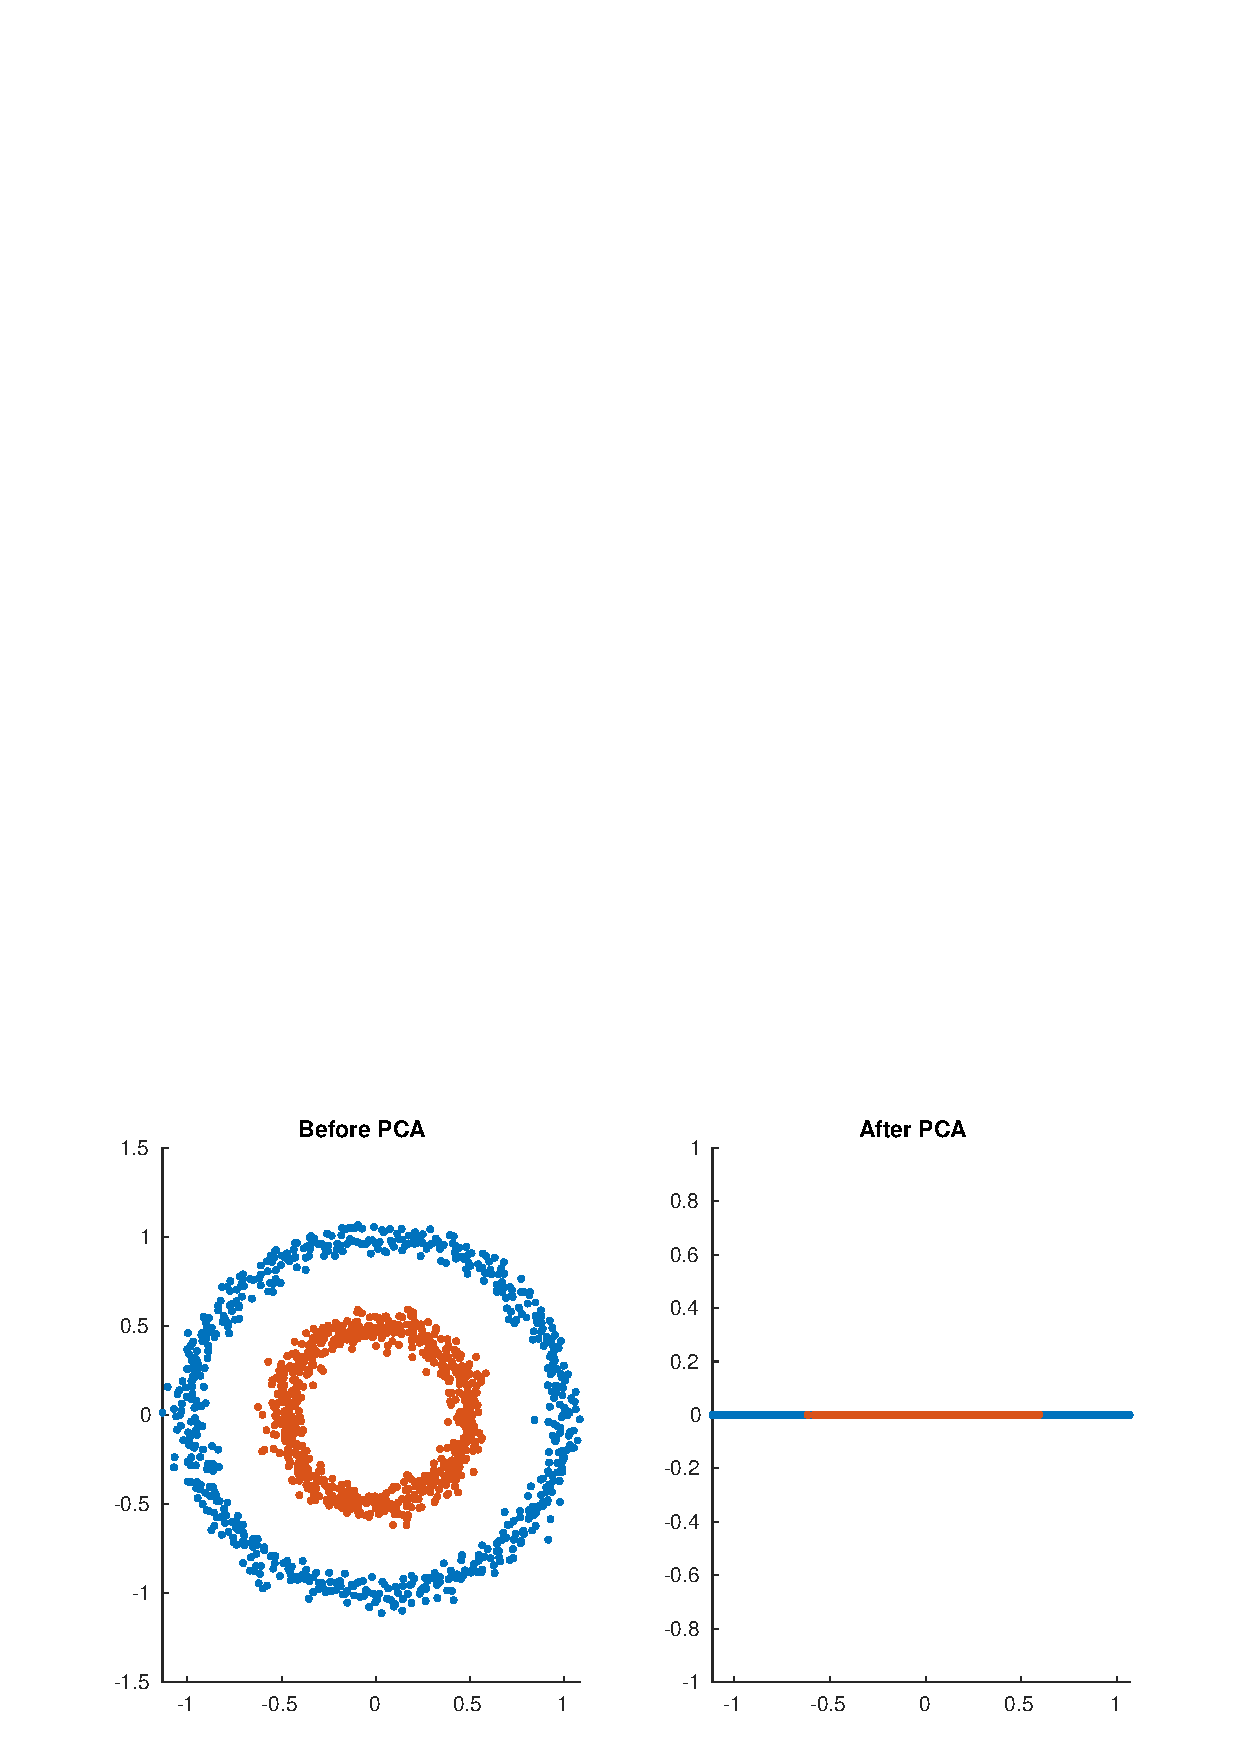
\includegraphics[width=\textwidth]{pic7.jpg}
			\end{figure}
			\item 
			مشکل۱: تفسیرناپذیری
		\begin{Large}
			\[\Phi(X)W\qquad\qquad\Phi(XW)\]
		\end{Large}
			\item 
			مشکل۲: عدم استفاده از برچسب داده‌ها در کاهش بُعد
		\end{itemize}
	\end{itemize}
\end{rawslide}
\begin{rawslide}
	\begin{itemize}
		\item \large\lr{IKDR}\normalsize
		\begin{itemize}
			\item 
			لزوم وجود یک معیار وابستگی
			\Large
			\[\max_W \;\;\mathrm{DEP}(XW,Y)\qquad \mathrm{s.t. } \;W^\top W = I\]
			\normalsize
			\item 
			معیار وابستگی
			\large\lr{HSIC}\normalsize
			
			\begin{equation*}
			\mathrm{MMD}(P, Q) = \norm{\mathbb{E}_{P}\left[ k(., X)\right] - \mathbb{E}_{Q}\left[ k(., X)\right]}_\mathcal{H}
			\end{equation*}
			\begin{equation*}
			\mathrm{HSIC}_k(X, Y) \triangleq \mathrm{MMD}_k(P_XP_Y, P_{XY})
			\end{equation*}
			\pause
			\item 
			تخمین 
			\large\lr{ HSIC}\normalsize
			از روی داده‌ها
			\begin{flalign*}
			\HSIC(XW, Y) &= \frac{1}{(n-1)^2} \tr (K_{XW}HK_YH)\\
			&= \frac{1}{(n-1)^2} \tr (HK_YHK_{XW})\\
			&= \frac{1}{(n-1)^2} \tr (\Gamma K_{XW})
			\end{flalign*}
		\end{itemize}
	\end{itemize}
\end{rawslide}
\begin{rawslide}
	\begin{itemize}
		\item 
		حلّ مسأله‌ی
		\large\lr{IKDR}\normalsize
		\begin{itemize}
			\item 
			یک مسأله‌ی بهینه‌سازی غیرمحدّب و به شدّت غیرخطّی
			\item 
			راه‌حل‌های قبلی موجود برای حلّ این مسأله
			\begin{itemize}
				\item \large\lr{Stiefel Manifold}\normalsize
				\item \large\lr{Grassman Manifold}\normalsize
				\item \large\lr{Dimension Growth}\normalsize
			\end{itemize}  
			\item 
			بهترین راه‌حل: الگوریتم 
			\large\lr{ Iterative Spectral Method (ISM)}\normalsize
			\begin{itemize}
				\item 
				پیاده‌سازی ساده‌تر
				\item 
				بسیار سریع‌تر از روش‌های قبلی
				\item 
				دچار مشکل‌ نشدن در نقاط زینی
				\item 
				تضمین تئوری فقط برای کرنل گاوسی
			\end{itemize}
		\item 
		هدف مقاله: تعمیم الگوریتم 
		\large\lr{ ISM}\normalsize
		به خانواده‌ی وسیع‌تری از کرنل‌ها
		\end{itemize}
	\end{itemize}
\end{rawslide}
\SecSlide[ISM]{\Huge\lr{Iterative Spectral Method}\normalsize}
\begin{rawslide}
	\subsection{ایده‌ی الگوریتم
	\large\lr{ ISM}\normalsize}		
		\begin{block}{تعریف کرنل‌
			\Large\lr{ ISM}\normalsize
		}
			\label{ISM-def}
			کرنل متقارن و مثبت معین
			$k(., .)$،
			یک کرنل 
			\lr{ISM}
			است، اگر دو بار مشتق‌پذیر باشد و برای آن داشته باشیم:
			\begin{equation}
			\forall \bx_i, \; \bx_j \in \R^d \;\;
			k(\bx_iW, \bx_jW) = f(\beta_{ij})
			\end{equation}
			که در آن
			\begin{equation}
			\beta_{ij} = a(\bx_i, \bx_j)^\top WW^\top b(\bx_i, \bx_j).
			\end{equation}
		\end{block}
	\begin{itemize}
		\item 
		مسأله‌ی بهینه‌سازی الگوریتم
		\large\lr{ IKDR}\normalsize:
		\[\max_W \;\; \tr(\Gamma K_{XW})\;\;\;\mathrm{s.t.}\;\;\;W^\top W=I\]
	\end{itemize}
\end{rawslide}
\begin{rawslide}
	مسأله‌ی بهینه‌سازی الگوریتم
	\large\lr{IKDR}\normalsize:\hfill
	$\max_W \;\; \tr(\Gamma K_{XW})\;\;\;\mathrm{s.t.}\;\;\;W^\top W=I$
	\begin{block}{قضیه}
		اگر
		\[-\frac{1}{2}\sum_{ij}{\Gamma_{ij} f'(\mathbf{a}^{T}WW^{T}\mathbf{b})} (\mathbf{b}\mathbf{a}^\top  + \mathbf{a}\mathbf{b}^\top )W - W \Lambda = 0.\]
		باشد، شرایط مرتبه‌ی اوّل مسأله‌ی بهینه‌سازی
		\large\lr{ IKDR}\normalsize
		برقرار می‌شود.
		این به آن معناست که 
		$W$
		باید شامل بردارهای ویژه‌ی ماتریس
		\[\Phi= -\frac{1}{2}\sum_{ij}{\Gamma_{ij} f'(\mathbf{a}^{T}WW^{T}\mathbf{b})} (\mathbf{b}\mathbf{a}^\top  + \mathbf{a}\mathbf{b}^\top )\]
		باشد. هم‌چنین اگر 
		$W$
		شامل بردارویژه‌های متناظر با کوچک‌ترین مقادیر ویژه‌ی 
		$\Phi$
		باشد، در شرایط مرتبه‌ی دوم مسأله‌ی بهینه‌سازی
		\large\lr{ IKDR}\normalsize
		هم صدق می‌کند.
		
	\end{block}
%		لاگرانژین مسأله:
%		\begin{align*}
%		\begin{split}
%		\mathcal{L}(W, \Lambda) = -\sum_{ij}
%		\Gamma_{ij} f(\mathbf{a}^{T}WW^{T}\mathbf{b}) 
%		- \tr[\Lambda(W^{T}W-I)]. \label{eq:Lagrangian}
%		\end{split}
%		\end{align*}
%		\item 
%		شرایط مرتبه‌ی اوّل:
%		\begin{flalign*}
%		\nabla_W \mathcal{L}(W, \Lambda) &= 
%		-\sum_{ij}{\Gamma_{ij} f'(\mathbf{a}^{T}WW^{T}\mathbf{b})} (\mathbf{b}\mathbf{a}^\top  + \mathbf{a}\mathbf{b}^\top )W - 2 W \Lambda= 0
%		\end{flalign*}
%		\begin{itemize}
%		\item 
%		تعریف می‌کنیم:
%		\[A = \mathbf{b}\mathbf{a}^\top  + \mathbf{a}\mathbf{b}^\top\]
%		\[\Psi_{i,j} = -\frac{1}{2}\Gamma_{i,j}f'(\mathbf{a}^{T}WW^{T}\mathbf{b})\]
%		\[\Phi = \sum_{i, j} \Psi_{ij}A_{i, j}\]
%		\item 
%		در نتیجه:
%		\[\Phi W = W \Lambda\]
%	\end{itemize}
\end{rawslide}
\begin{rawslide}
	\begin{itemize}
		\item 
		الگوریتم
		\large\lr{ISM}\normalsize:
		\begin{latin}
			\setstretch{1.5}
			\begin{algorithm}[H]
				\SetAlgoLined
				\KwIn{Data $X$, kernel, Subspace Dimension $q$}
				\KwOut{Projected subspace $W$} 
				\textbf{Initialization:} Initialize $\Phi_0$.
				
				Set $W_0$ to Dominant Eigenvectors of  of $\Phi_0$
				
				\While{ $||\Lambda_i - \Lambda_{i-1}||_2/||\Lambda_i||_2 < \delta$ }{
				
				Compute $\Phi$ with $W_{k-1}$
				
				Set $W_k$ to Dominant Eigenvectors of $\Phi$
			}
				
				\caption{ISM Algorithm}
				\label{alg:ism}
			\end{algorithm}   
		\end{latin}
		\normalsize
		\item 
		انتخاب یک شرط اوّلیّه‌ی مناسب:
		$\Phi_0$
	\end{itemize}
	\pause
	\begin{block}{قضیه}
		هر ترکیب خطّی با ضرایب مثبت ازکرنل‌های
		\large\lr{ISM}\normalsize،
		خود یک کرنل 
			\large\lr{ ISM}\normalsize
			است و ماتریس
			$\Phi$
			آن، از ترکیب خطّی ماتریس‌های
			$\Phi$
			کرنل‌های اوّلیه با همان ضرایب به دست می‌آید.
	\end{block}
\end{rawslide}
\SecSlide{کاربردها}
\begin{rawslide}
	\subsection{کاربردهای الگوریتم
	\Large\lr{ISM}\normalsize}
	\begin{itemize}
		\item 
		مسأله‌ی کاهش بُعد با نظارت
		\large\lr{(Supervised Dimension Reduction)}\normalsize
		\item 
		مسأله‌ی کاهش بُعد بدون نظارت
		\large\lr{(Unsupervised Dimension Reduction)}\normalsize
		\item 
		مسأله‌ی کاهش بُعد با نظارت ناقص
		\large\lr{(Semi-Supervised Dimension Reduction)}\normalsize
		\item 
		مسأله‌ی کاهش بعد جایگزین
		\large\lr{(Alternative Clustering)}
	\end{itemize}
\end{rawslide}
\SecSlide{شبیه‌سازی}
\begin{rawslide}
	
\end{rawslide}


\SecSlide{مراجع}
\begin{rawslide}
	\begin{tblock}
		\nocite{*}
		\bibliographystyle{unsrt-fa}
		\bibliography{Reference1}
	\end{tblock}
\end{rawslide}
\begin{comment}
\begin{rawslide}

\begin{thebibliography}{99}\vspace*{1.5cm}
\begin{tblock}
\begin{LTRbibitems}
\resetlatinfont
%مراجع لاتین👇

%\begin{flushleft}
\bibitem{MC}M. Crainic, R. Fernandes, Integrability of Lie brackets, \emph{Ann. of Math} \textbf{157} (2003) 575-620.

\bibitem{FB}Gh. Fasihi Ramandi, N. Boroojerdian, Forces Unification in The Framework of Transitive
Lie Algebroids,  \emph{Int.J.Theor.Phys} \textbf{54} (2015) 1581-1593.

\bibitem{CI}C. Ida, P. Popescu, On almost complex Lie algebroids, \emph{Mediterr. J. Math} (2015) 1-22.

\bibitem{RN} R. Nest, B. Tsygan, Deformations of symplectic Lie algebroids, deformations of holomorphic symplectic structures, and index theorems \emph{Asian J. Math.}, \textbf{5} (2001), 599–635.

%\end{flushleft}

\end{LTRbibitems}\end{tblock}
\end{thebibliography}\end{rawslide}
\end{comment}

